%%%%%%%%%%%%%%%%%%%%%%%%%%%%%%%%%%%%%%%%%
% Masters/Doctoral Thesis 
% LaTeX Template
% Version 2.5 (27/8/17)
%
% This template was downloaded from:
% http://www.LaTeXTemplates.com
%
% Version 2.x major modifications by:
% Vel (vel@latextemplates.com)
%
% This template is based on a template by:
% Steve Gunn (http://users.ecs.soton.ac.uk/srg/softwaretools/document/templates/)
% Sunil Patel (http://www.sunilpatel.co.uk/thesis-template/)
%
% Template license:
% CC BY-NC-SA 3.0 (http://creativecommons.org/licenses/by-nc-sa/3.0/)
%
%%%%%%%%%%%%%%%%%%%%%%%%%%%%%%%%%%%%%%%%%

%----------------------------------------------------------------------------------------
%	PACKAGES AND OTHER DOCUMENT CONFIGURATIONS
%----------------------------------------------------------------------------------------

\documentclass[
11pt, % The default document font size, options: 10pt, 11pt, 12pt
%oneside, % Two side (alternating margins) for binding by default, uncomment to switch to one side
english, % ngerman for German
singlespacing, % Single line spacing, alternatives: onehalfspacing or doublespacing
%draft, % Uncomment to enable draft mode (no pictures, no links, overfull hboxes indicated)
%nolistspacing, % If the document is onehalfspacing or doublespacing, uncomment this to set spacing in lists to single
%liststotoc, % Uncomment to add the list of figures/tables/etc to the table of contents
%toctotoc, % Uncomment to add the main table of contents to the table of contents
%parskip, % Uncomment to add space between paragraphs
%nohyperref, % Uncomment to not load the hyperref package
headsepline, % Uncomment to get a line under the header
%chapterinoneline, % Uncomment to place the chapter title next to the number on one line
%consistentlayout, % Uncomment to change the layout of the declaration, abstract and acknowledgements pages to match the default layout
]{MastersDoctoralThesis} % The class file specifying the document structure

\usepackage[utf8]{inputenc} % Required for inputting international characters
\usepackage[T1]{fontenc} % Output font encoding for international characters

\usepackage{mathpazo} % Use the Palatino font by default

\usepackage[backend=bibtex,style=authoryear,natbib=true]{biblatex} % Use the bibtex backend with the authoryear citation style (which resembles APA)

\addbibresource{example.bib} % The filename of the bibliography

\usepackage[autostyle=true]{csquotes} % Required to generate language-dependent quotes in the bibliography

%----------------------------------------------------------------------------------------
%	MARGIN SETTINGS
%----------------------------------------------------------------------------------------

\geometry{
	paper=a4paper, % Change to letterpaper for US letter
	inner=2.5cm, % Inner margin
	outer=3.8cm, % Outer margin
	bindingoffset=.5cm, % Binding offset
	top=1.5cm, % Top margin
	bottom=1.5cm, % Bottom margin
	%showframe, % Uncomment to show how the type block is set on the page
}

%----------------------------------------------------------------------------------------
%	THESIS INFORMATION
%----------------------------------------------------------------------------------------

\thesistitle{Intelligence artificiel} % Your thesis title, this is used in the title and abstract, print it elsewhere with \ttitle
\supervisor{Pr. Mautor \textsc{Thierry}} % Your supervisor's name, this is used in the title page, print it elsewhere with \supname
\examiner{} % Your examiner's name, this is not currently used anywhere in the template, print it elsewhere with \examname
\degree{Master 1 informatique} % Your degree name, this is used in the title page and abstract, print it elsewhere with \degreename
\author{Arnaud \textsc{Dufour \\ Nicolas \textsc{Carbonnier}\\ Jean-Charles \textsc{Sottas}\\
Thibaud \textsc{Larcher}}} % Your name, this is used in the title page and abstract, print it elsewhere with \authorname
\addresses{} % Your address, this is not currently used anywhere in the template, print it elsewhere with \addressname

\subject{Informatique} % Your subject area, this is not currently used anywhere in the template, print it elsewhere with \subjectname
\keywords{} % Keywords for your thesis, this is not currently used anywhere in the template, print it elsewhere with \keywordnames
\university{\href{http://www.uvsq.fr/universite-de-versailles-saint-quentin-en-yvelines-363917.kjsp}{UVSQ}} % Your university's name and URL, this is used in the title page and abstract, print it elsewhere with \univname
% \department{\href{http://department.university.com}{Department or School Name}} % Your department's name and URL, this is used in the title page and abstract, print it elsewhere with \deptname
% \group{\href{http://researchgroup.university.com}{Research Group Name}} % Your research group's name and URL, this is used in the title page, print it elsewhere with \groupname
% \faculty{\href{http://faculty.university.com}{Faculty Name}} % Your faculty's name and URL, this is used in the title page and abstract, print it elsewhere with \facname

\AtBeginDocument{
\hypersetup{pdftitle=\ttitle} % Set the PDF's title to your title
\hypersetup{pdfauthor=\authorname} % Set the PDF's author to your name
\hypersetup{pdfkeywords=\keywordnames} % Set the PDF's keywords to your keywords
}

\begin{document}

\frontmatter % Use roman page numbering style (i, ii, iii, iv...) for the pre-content pages

\pagestyle{plain} % Default to the plain heading style until the thesis style is called for the body content

%----------------------------------------------------------------------------------------
%	TITLE PAGE
%----------------------------------------------------------------------------------------

\begin{titlepage}
\begin{center}

\vspace*{.06\textheight}
{\scshape\LARGE \univname\par}\vspace{1.5cm} % University name
\textsc{\Large TER}\\[0.5cm] % Thesis type

\HRule \\[0.4cm] % Horizontal line
{\huge \bfseries \ttitle\par}\vspace{0.4cm} % Thesis title
\HRule \\[1.5cm] % Horizontal line
 
\begin{minipage}[t]{0.4\textwidth}
\begin{flushleft} \large
\emph{Auteurs:}\\
{\authorname} % Author name - remove the \href bracket to remove the link
\end{flushleft}
\end{minipage}
\begin{minipage}[t]{0.4\textwidth}
\begin{flushright} \large
\emph{Superviseur:} \\
{\supname} % Supervisor name - remove the \href bracket to remove the link  
\end{flushright}
\end{minipage}\\[3cm]
 
\vfill

\large \textit{Compte rendu du TER pour le \\ \degreename}\\[0.3cm] % University requirement text
\textit{in the}\\[0.4cm]
% \groupname\\\deptname\\[2cm] % Research group name and department name
 
\vfill

{\large \today}\\[4cm] % Date
%\includegraphics{Logo} % University/department logo - uncomment to place it
 
\vfill
\end{center}
\end{titlepage}

%----------------------------------------------------------------------------------------
%	DECLARATION PAGE
%----------------------------------------------------------------------------------------


%----------------------------------------------------------------------------------------
%	QUOTATION PAGE
%----------------------------------------------------------------------------------------

\vspace*{0.2\textheight}

\noindent\enquote{\itshape La création de l'intelligence artificielle serait le plus grand événement de l'histoire \- de l'humanité.\\Mais il pourrait aussi être l'ultime.}\bigbreak

\hfill Stephen Hawking

%----------------------------------------------------------------------------------------
%	LIST OF CONTENTS/FIGURES/TABLES PAGES
%----------------------------------------------------------------------------------------

\tableofcontents % Prints the main table of contents

% \listoffigures % Prints the list of figures

% \listoftables % Prints the list of tables

%----------------------------------------------------------------------------------------
%	ABBREVIATIONS
%----------------------------------------------------------------------------------------

% \begin{abbreviations}{ll} % Include a list of abbreviations (a table of two columns)

% \textbf{LAH} & \textbf{L}ist \textbf{A}bbreviations \textbf{H}ere\\
% \textbf{WSF} & \textbf{W}hat (it) \textbf{S}tands \textbf{F}or\\

% \end{abbreviations}

%----------------------------------------------------------------------------------------
%	PHYSICAL CONSTANTS/OTHER DEFINITIONS
%----------------------------------------------------------------------------------------

% \begin{constants}{lr@{${}={}$}l} % The list of physical constants is a three column table

% The \SI{}{} command is provided by the siunitx package, see its documentation for instructions on how to use it

% Speed of Light & $c_{0}$ & \SI{2.99792458e8}{\meter\per\second} (exact)\\
%Constant Name & $Symbol$ & $Constant Value$ with units\\

% \end{constants}

%----------------------------------------------------------------------------------------
%	SYMBOLS
%----------------------------------------------------------------------------------------

% \begin{symbols}{lll} % Include a list of Symbols (a three column table)

% $a$ & distance & \si{\meter} \\
% $P$ & power & \si{\watt} (\si{\joule\per\second}) \\
% %Symbol & Name & Unit \\

% \addlinespace % Gap to separate the Roman symbols from the Greek

% $\omega$ & angular frequency & \si{\radian} \\

% \end{symbols}

%----------------------------------------------------------------------------------------
%	DEDICATION
%----------------------------------------------------------------------------------------

% \dedicatory{For/Dedicated to/To my\ldots} 

%----------------------------------------------------------------------------------------
%	THESIS CONTENT - CHAPTERS
%----------------------------------------------------------------------------------------

\mainmatter % Begin numeric (1,2,3...) page numbering

\pagestyle{thesis} % Return the page headers back to the "thesis" style

% Include the chapters of the thesis as separate files from the Chapters folder
% Uncomment the lines as you write the chapters

% Chapter 1

\chapter{Introduction} % Main chapter title

\label{Chapter1} % For referencing the chapter elsewhere, use \ref{Chapter1} 

%----------------------------------------------------------------------------------------

% Define some commands to keep the formatting separated from the content 
\newcommand{\keyword}[1]{\textbf{#1}}
\newcommand{\tabhead}[1]{\textbf{#1}}
\newcommand{\code}[1]{\texttt{#1}}
\newcommand{\file}[1]{\texttt{\bfseries#1}}
\newcommand{\option}[1]{\texttt{\itshape#1}}

%----------------------------------------------------------------------------------------

Ce projet a pour but de nous initier à la création d'intelligences artificielles.\\Ces dernières permettant la résolution de problèmes complexes en un minimum de temps.\\
Elles vont nous permettrent de jouer avec différentes approches tactique du jeu.\\
Nous appliquerons ces IA sur un jeu de société appelé "Kingdomino".\\ \\
Dans un premier temps, nous expliquerons le jeu de société - règles et programmation - et nous l'utiliserons avec un exemple puis nous arborderons le sujet des Intelligences Artificielle - fonctionnement et programmation - pour enfin finir sur la résolution du jeu.


% Chapter 2

\chapter{Kingdomino} % Main chapter title

\label{Chapter2} % For referencing the chapter elsewhere, use \ref{Chapter1}

\section{Le jeu de société}
Le jeu Kingdomino est un jeu de société de prise de territoire utilisant des tuiles ou dominos de type de terrains différents. Le jeu se joue de 2 à 4 joueurs.\\
Le jeu est composé de :
\begin{itemize}
    \item 4 tuiles de départ neutre.
    \item 48 dominos avec une face paysage et une face numérotée.
    \item 8 rois de 4 couleurs différentes.
\end{itemize}

\begin{center}
  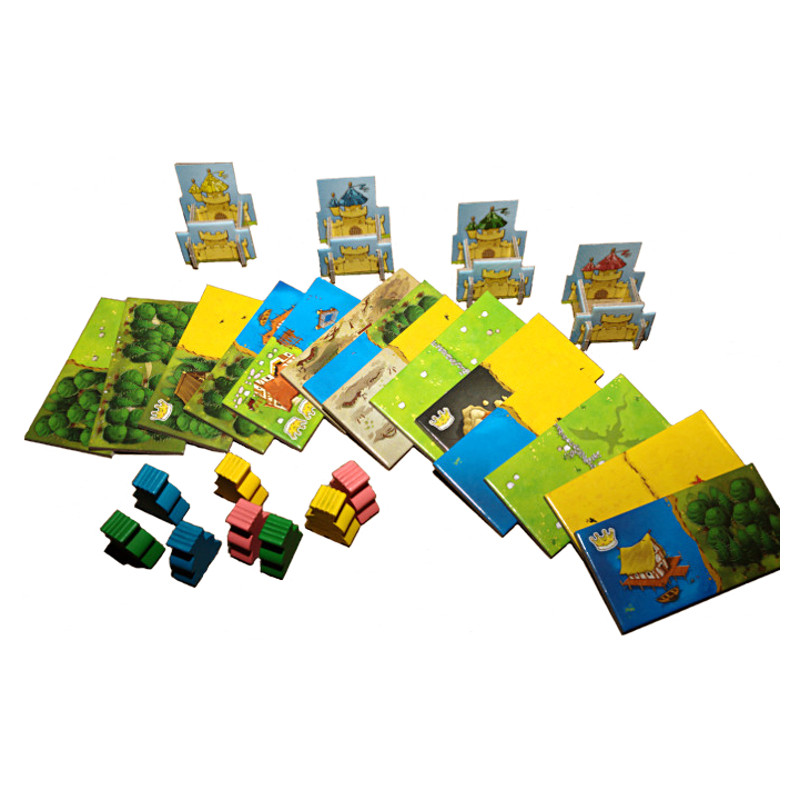
\includegraphics[scale=0.5]{Figures/jeuking}
  \caption{Kingdomino}
\end{center}

\subsection{But du jeu}
Le but du jeu est de connecter astucieusement vos dominos afin de construire le royaume de $5 \times 5$ cases le plus prestigieux et de marquer le plus de points possible.

%----------------------------------------------------------------------------------------
\newpage
\section{Les règles}

Les règles du jeu ne sont pas très compliquées mais soyez attentif :

\subsection{Le commencement}
Pour un jeu à 2 joueurs, on utilisera que 24 dominos.\\
Pour un jeu à 3 joueurs, on utilisera 36 dominos.\\
Et enfin, pour un jeu à 4 joueurs, on utilisera les 48 dominos.\\\\
L'ordre du premier tour de jeu est déterminé par de l'aléatoire, c'est un choix de notre part. Devant les joueurs il y a un pioche de tuiles, 4 par tour si le jeu se joue à 2 ou 4 joueurs sinon il y aura 3 tuiles devant les joueurs. Elles sont rangées par ordre croissant de numéro de tuile.\\
Chacun leur tour, les joueurs vont choisir quel domino ils veulent prendre parmis les 4  proposés (ou 3 si jeu à 3 joueurs) grâce a leur "roi", qu'ils vont placer sur le domino qu'ils convoitent, afin de compléter leur royaume et marquer un maximum de points.\\
\\
Exemple de pioche de tuile à 2 ou 4 joueurs :\\

\begin{center}
  
\includegraphics[scale=0.5]{Figures/tuiledistrib.png}
  \caption{tuile1}
\end{center}
\\ \\
Imaginons que le premier tour de jeu se passe comme cela :\\

\begin{center}
  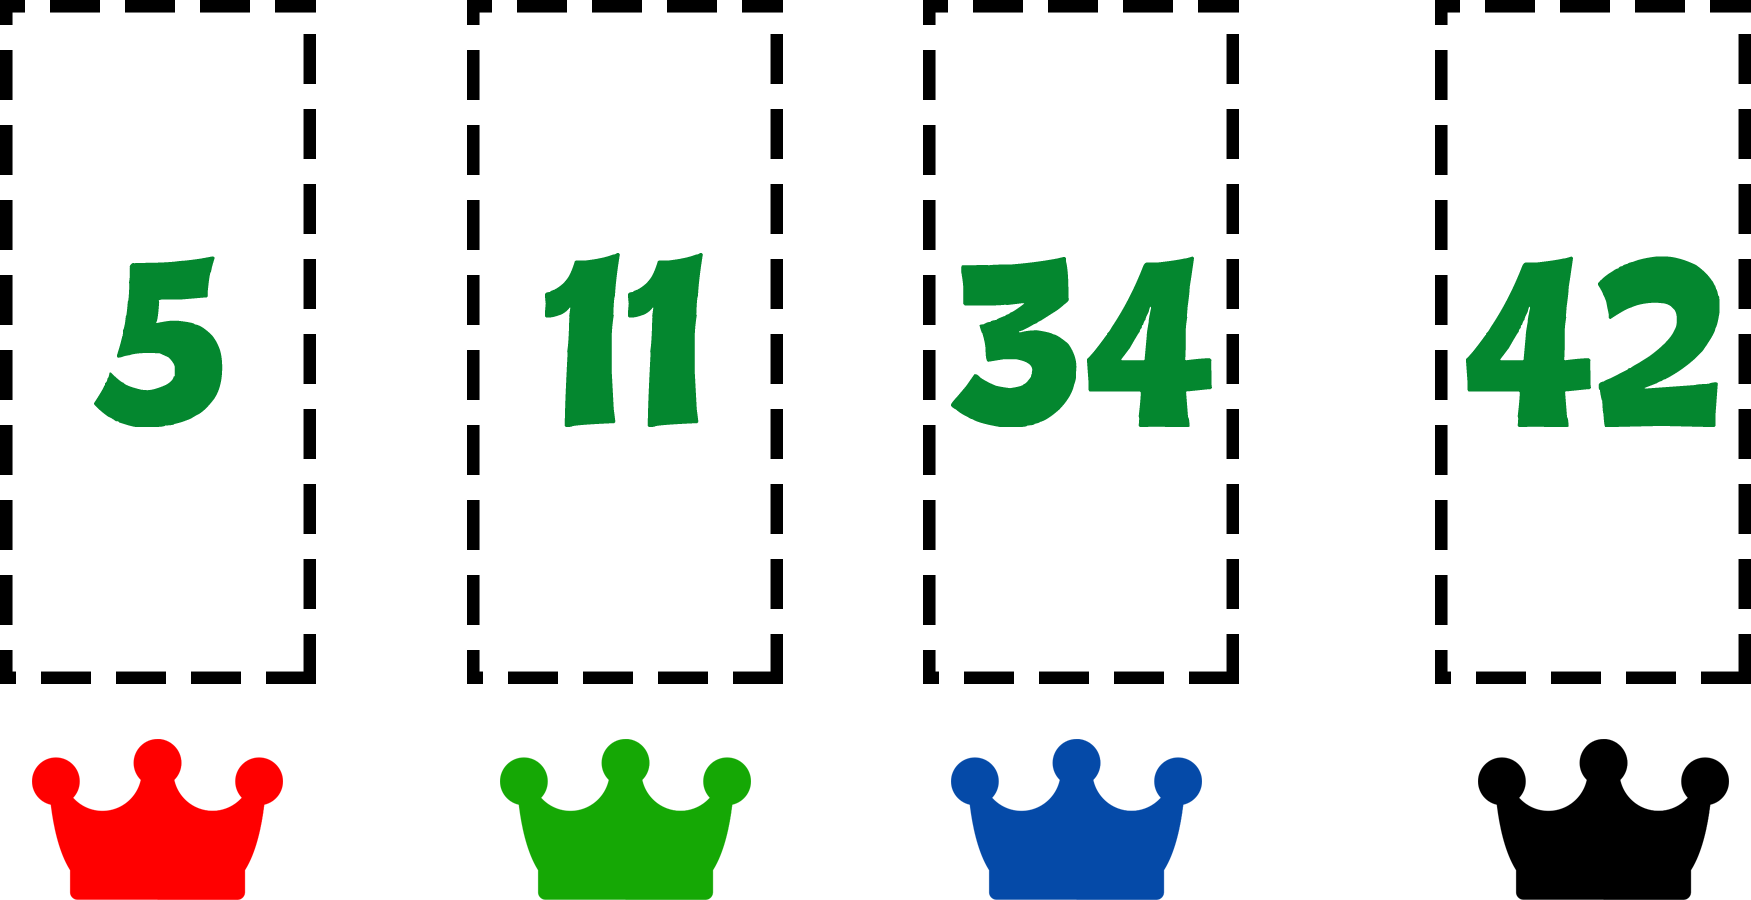
\includegraphics[scale=0.5]{Figures/tuileroi.png}
  \caption{tuile2}
\end{center}
\\ \\
Alors le roi  
\includegraphics[scale=0.3]{Figures/roirouge.png} sera le premier a jouer au tour suivant puisqu'il a choisi la tuile avec le numéro le plus petit entre les 4.
Logiquement, en deuxième c'est le roi 
\includegraphics[scale=0.3]{Figures/roivert.png} puis le roi 
\includegraphics[scale=0.3]{Figures/roibleu.png} et enfin le dernier le roi 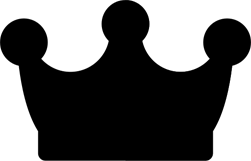
\includegraphics[scale=0.3]{Figures/roinoir.png}.\\
\\
Ainsi de suite jusqu'a la fin du jeu.

\newpage
\subsection{La connexion des tuiles}

Les joueurs doivent donc construire un royaume de $5 \times 5$ cases (un domino étant constitué de 2 cases).\\
Pour pouvoir poser son domino, le joueur doit :
\begin{itemize}
    \item Soit le connecter à son chateau de départ, qui est considéré comme une tuile joker (n'importe quel paysage peut être collé à ce domino).
\end{itemize}
\begin{center}
  
\includegraphics[scale=0.5]{Figures/tuilechateau.png}
  \caption{tuile3}
\end{center}
\begin{itemize}
    \item Soit le connecter à un autre domino en faisant correspondre au minimum 1 paysage (horizontalement ou verticalement uniquement).
\end{itemize}
\begin{center}
  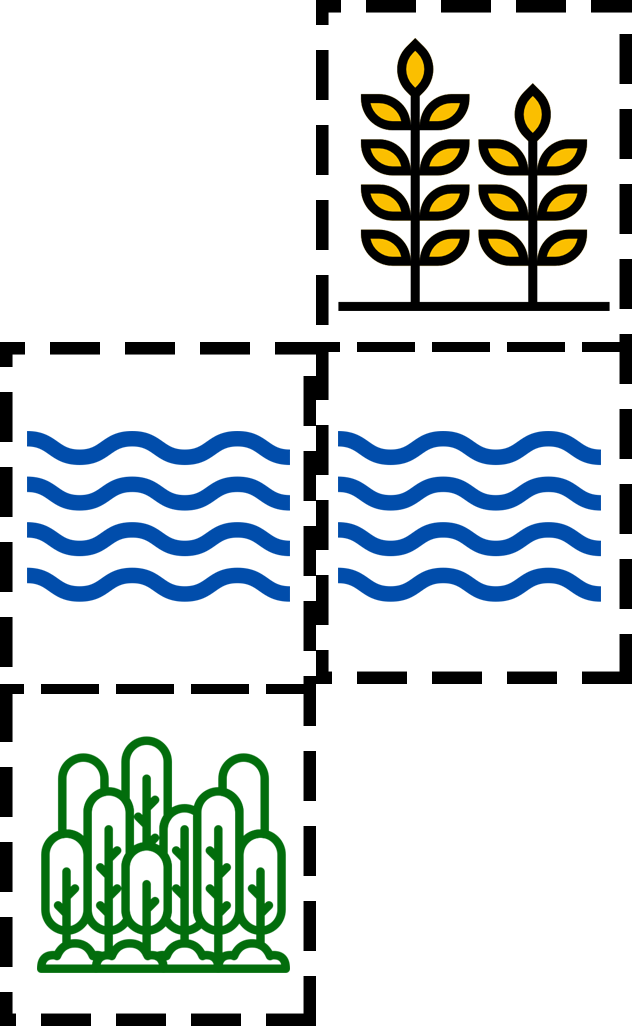
\includegraphics[scale=0.5]{Figures/2tuiles.png}
  \caption{tuile4}
\end{center}
\\
Dans le cas où il est impossible de venir ajouter un domino à son royaume en respectant les règles ci-dessus, le domino est défaussé et ne rapportera aucun point.\\\\
Tous les dominos doivent tenir dans un espace de $ 5 \times 5$ cases.\\\\
En cas de mauvaise anticipation, un à plusieurs dominos pourraient ne plus être exploitables et seront défaussés. Ils ne rapporteront alors aucun point.

\newpage
\subsection{Le fin du jeu}

Lorsque les derniers dominos sont placés en ligne au milieu de la table, les joueurs jouent un dernier tour normalement.\\
Chaque joueur devrait alors avoir devant lui un royaume de $5 \times 5$ cases. (Certains royaumes peuvent être incomplets si le joueur a été obligé de défausser des dominos.)\\
Chaque joueur va calculer les points de prestige de son royaume de la façon suivante :
\begin{itemize}
    \item Un royaume est constitué de différents \textbf{DOMAINES} (groupe de cases connectées horizontalement ou verticalement du même type de terrain).
    \item Chaque domaine rapporte autant de points de prestige que son \textbf{NOMBRE DE CASES} multiplié par le \textbf{NOMBRE DE COURONNES} présentes sur le domaine.
    \item Il peut y avoir plusieurs domaine du même type de terrain dans un même royaume.
    \item Un domaine sans couronne ne rapport aucun point.
    \item Chaque joueur additionne les points rapportés par chacun de ses domaines, le résultat de cette addition lui donne son score final.
    \item Le joueur qui a le plus haut score gagne la partie.
    \item En cas d'égalité, le joueur qui a construit le domaine le plus étendus, remporte la partie. Si cela ne suffit pas, c'est celui qui a le plus de couronne et si cela ne suffit toujours pas alors ils ont gagné tous les deux.
\end{itemize}

\begin{center}
  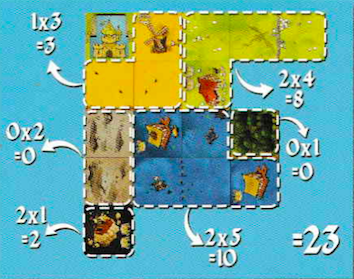
\includegraphics[scale=0.5]{Figures/exFindeJeu.png}
  \caption{FinDeJeu}
\end{center}

\subsection{Règles additionnelles et optionnelles}

Il existe des règles additionnelles et optionnelles pour des modes de jeu différents mais nous sommes rester dans les limites des règles du jeu classique.

%----------------------------------------------------------------------------------------
%% Chapter 2

\chapter{Kingdomino} % Main chapter title

\label{Chapter2} % For referencing the chapter elsewhere, use \ref{Chapter1}

\section{Le jeu de société}
Le jeu Kingdomino est un jeu de société de prise de territoire utilisant des tuiles ou dominos de type de terrains différents. Le jeu se joue de 2 à 4 joueurs.\\
Le jeu est composé de :
\begin{itemize}
    \item 4 tuiles de départ neutre.
    \item 48 dominos avec une face paysage et une face numérotée.
    \item 8 rois de 4 couleurs différentes.
\end{itemize}

\begin{center}
  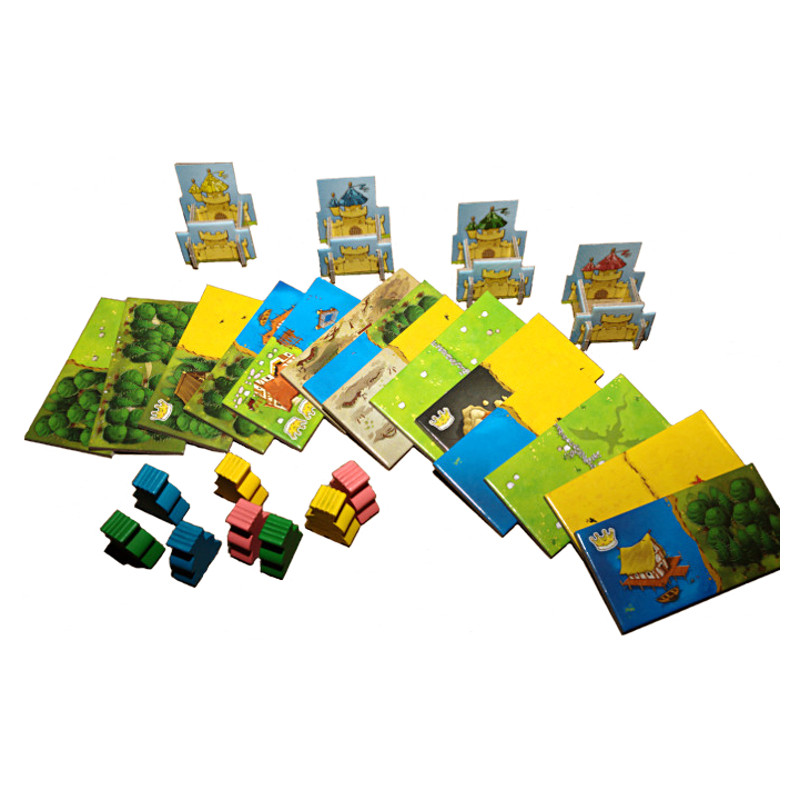
\includegraphics[scale=0.5]{Figures/jeuking}
  \caption{Kingdomino}
\end{center}

\subsection{But du jeu}
Le but du jeu est de connecter astucieusement vos dominos afin de construire le royaume de $5 \times 5$ cases le plus prestigieux et de marquer le plus de points possible.

%----------------------------------------------------------------------------------------
\newpage
\section{Les règles}

Les règles du jeu ne sont pas très compliquées mais soyez attentif :

\subsection{Le commencement}
Pour un jeu à 2 joueurs, on utilisera que 24 dominos.\\
Pour un jeu à 3 joueurs, on utilisera 36 dominos.\\
Et enfin, pour un jeu à 4 joueurs, on utilisera les 48 dominos.\\\\
L'ordre du premier tour de jeu est déterminé par de l'aléatoire, c'est un choix de notre part. Devant les joueurs il y a un pioche de tuiles, 4 par tour si le jeu se joue à 2 ou 4 joueurs sinon il y aura 3 tuiles devant les joueurs. Elles sont rangées par ordre croissant de numéro de tuile.\\
Chacun leur tour, les joueurs vont choisir quel domino ils veulent prendre parmis les 4  proposés (ou 3 si jeu à 3 joueurs) grâce a leur "roi", qu'ils vont placer sur le domino qu'ils convoitent, afin de compléter leur royaume et marquer un maximum de points.\\
\\
Exemple de pioche de tuile à 2 ou 4 joueurs :\\

\begin{center}
  
\includegraphics[scale=0.5]{Figures/tuiledistrib.png}
  \caption{tuile1}
\end{center}
\\ \\
Imaginons que le premier tour de jeu se passe comme cela :\\

\begin{center}
  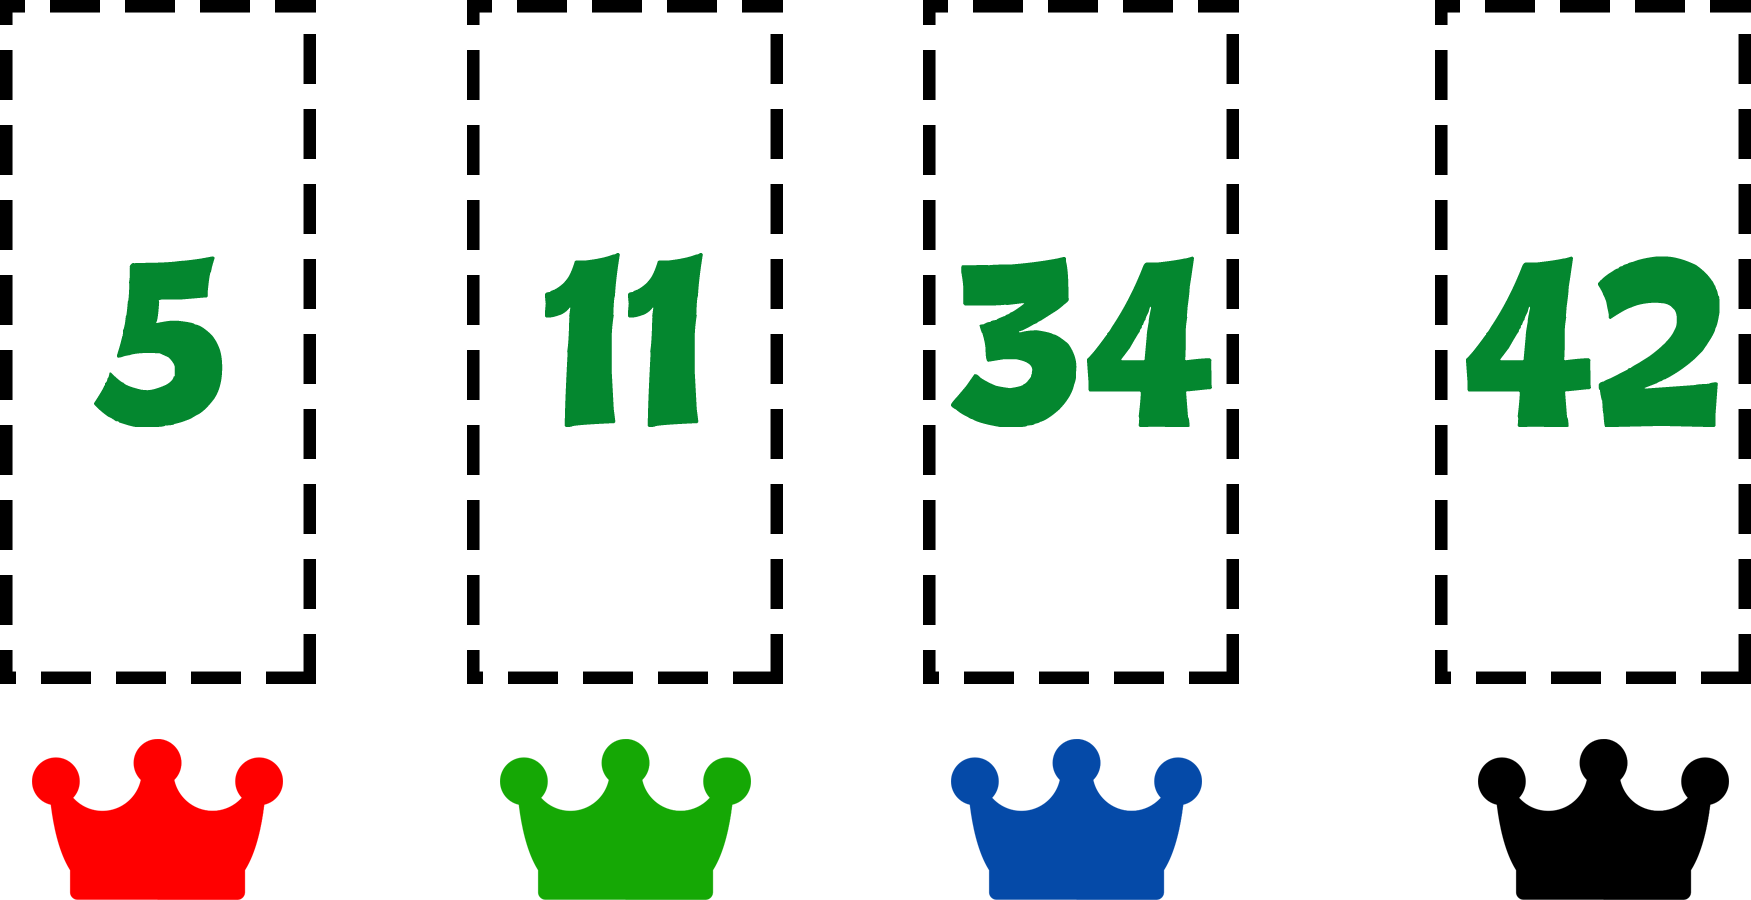
\includegraphics[scale=0.5]{Figures/tuileroi.png}
  \caption{tuile2}
\end{center}
\\ \\
Alors le roi  
\includegraphics[scale=0.3]{Figures/roirouge.png} sera le premier a jouer au tour suivant puisqu'il a choisi la tuile avec le numéro le plus petit entre les 4.
Logiquement, en deuxième c'est le roi 
\includegraphics[scale=0.3]{Figures/roivert.png} puis le roi 
\includegraphics[scale=0.3]{Figures/roibleu.png} et enfin le dernier le roi 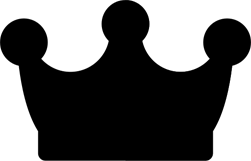
\includegraphics[scale=0.3]{Figures/roinoir.png}.\\
\\
Ainsi de suite jusqu'a la fin du jeu.

\newpage
\subsection{La connexion des tuiles}

Les joueurs doivent donc construire un royaume de $5 \times 5$ cases (un domino étant constitué de 2 cases).\\
Pour pouvoir poser son domino, le joueur doit :
\begin{itemize}
    \item Soit le connecter à son chateau de départ, qui est considéré comme une tuile joker (n'importe quel paysage peut être collé à ce domino).
\end{itemize}
\begin{center}
  
\includegraphics[scale=0.5]{Figures/tuilechateau.png}
  \caption{tuile3}
\end{center}
\begin{itemize}
    \item Soit le connecter à un autre domino en faisant correspondre au minimum 1 paysage (horizontalement ou verticalement uniquement).
\end{itemize}
\begin{center}
  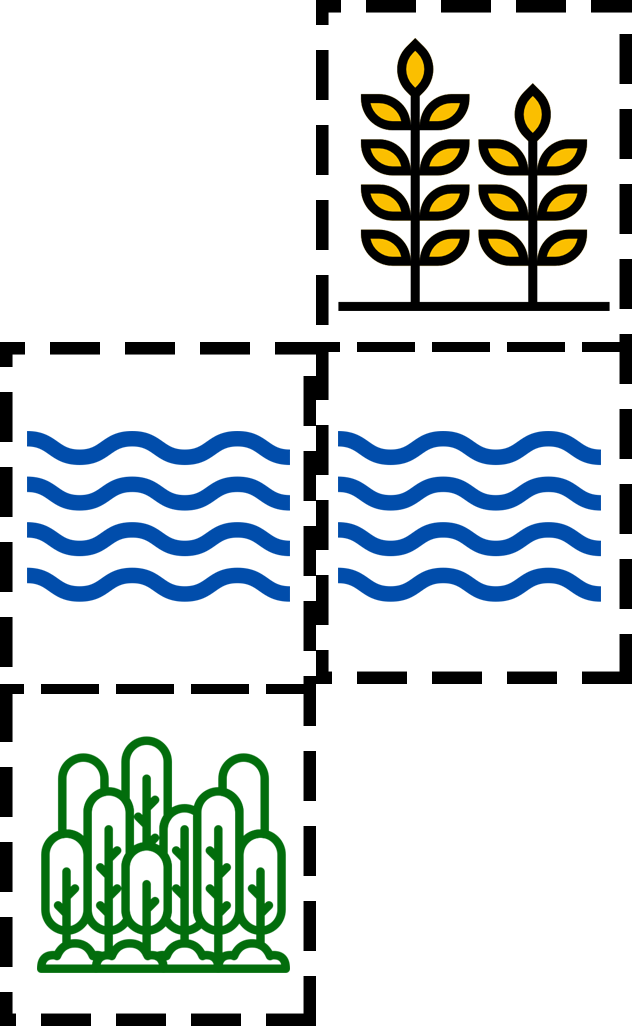
\includegraphics[scale=0.5]{Figures/2tuiles.png}
  \caption{tuile4}
\end{center}
\\
Dans le cas où il est impossible de venir ajouter un domino à son royaume en respectant les règles ci-dessus, le domino est défaussé et ne rapportera aucun point.\\\\
Tous les dominos doivent tenir dans un espace de $ 5 \times 5$ cases.\\\\
En cas de mauvaise anticipation, un à plusieurs dominos pourraient ne plus être exploitables et seront défaussés. Ils ne rapporteront alors aucun point.

\newpage
\subsection{Le fin du jeu}

Lorsque les derniers dominos sont placés en ligne au milieu de la table, les joueurs jouent un dernier tour normalement.\\
Chaque joueur devrait alors avoir devant lui un royaume de $5 \times 5$ cases. (Certains royaumes peuvent être incomplets si le joueur a été obligé de défausser des dominos.)\\
Chaque joueur va calculer les points de prestige de son royaume de la façon suivante :
\begin{itemize}
    \item Un royaume est constitué de différents \textbf{DOMAINES} (groupe de cases connectées horizontalement ou verticalement du même type de terrain).
    \item Chaque domaine rapporte autant de points de prestige que son \textbf{NOMBRE DE CASES} multiplié par le \textbf{NOMBRE DE COURONNES} présentes sur le domaine.
    \item Il peut y avoir plusieurs domaine du même type de terrain dans un même royaume.
    \item Un domaine sans couronne ne rapport aucun point.
    \item Chaque joueur additionne les points rapportés par chacun de ses domaines, le résultat de cette addition lui donne son score final.
    \item Le joueur qui a le plus haut score gagne la partie.
    \item En cas d'égalité, le joueur qui a construit le domaine le plus étendus, remporte la partie. Si cela ne suffit pas, c'est celui qui a le plus de couronne et si cela ne suffit toujours pas alors ils ont gagné tous les deux.
\end{itemize}

\begin{center}
  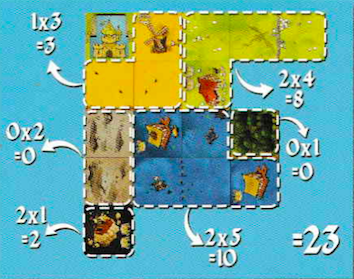
\includegraphics[scale=0.5]{Figures/exFindeJeu.png}
  \caption{FinDeJeu}
\end{center}

\subsection{Règles additionnelles et optionnelles}

Il existe des règles additionnelles et optionnelles pour des modes de jeu différents mais nous sommes rester dans les limites des règles du jeu classique.

%---------------------------------------------------------------------------------------- 
%% Chapter 3

\chapter{Conception du jeu et développement des IA} % Main chapter title

\label{Chapter3} % Change X to a consecutive number; for referencing this chapter elsewhere, use \ref{ChapterX}

%----------------------------------------------------------------------------------------
%	SECTION 1
%----------------------------------------------------------------------------------------

\section{Introduction}

Notre sujet de TER était donc de développer plusieurs IA afin de pouvoir les affronter lors d'une partie de Kingdomino ou même de les faire s'affronter entre elles.\\
Nous avons dans un premier temps programmer le jeu Kingdomino lui même. Puis nous avons ensuite réfléchi pour le developpement des différentes IA. 

\section{Structure du jeu}

Pour le développement de notre jeu et des IA, nous avons décider de choisir comme langage de programmation le Python car c'est un langage plus adapté pour le développement d'IA.\\
Nous avons également choisi le logiciel Processing, particulièrement adapté pour toute la partie graphique.

\subsection{Implémentation}
Morbi rutrum odio eget arcu adipiscing sodales. Aenean et purus a est pulvinar pellentesque. Cras in elit neque, quis varius elit. Phasellus fringilla, nibh eu tempus venenatis, dolor elit posuere quam, quis adipiscing urna leo nec orci. Sed nec nulla auctor odio aliquet consequat. Ut nec nulla in ante ullamcorper aliquam at sed dolor. Phasellus fermentum magna in augue gravida cursus. Cras sed pretium lorem. Pellentesque eget ornare odio. Proin accumsan, massa viverra cursus pharetra, ipsum nisi lobortis velit, a malesuada dolor lorem eu neque.

\section{Structure des IA}
Nunc posuere quam at lectus tristique eu ultrices augue venenatis. Vestibulum ante ipsum primis in faucibus orci luctus et ultrices posuere cubilia Curae; Aliquam erat volutpat. Vivamus sodales tortor eget quam adipiscing in vulputate ante ullamcorper. Sed eros ante, lacinia et sollicitudin et, aliquam sit amet augue. In hac habitasse platea dictumst.

\subsection{Implémentation}
Sed ullamcorper quam eu nisl interdum at interdum enim egestas. Aliquam placerat justo sed lectus lobortis ut porta nisl porttitor. Vestibulum mi dolor, lacinia molestie gravida at, tempus vitae ligula. Donec eget quam sapien, in viverra eros. Donec pellentesque justo a massa fringilla non vestibulum metus vestibulum. Vestibulum in orci quis felis tempor lacinia. Vivamus ornare ultrices facilisis. Ut hendrerit volutpat vulputate. Morbi condimentum venenatis augue, id porta ipsum vulputate in. Curabitur luctus tempus justo. Vestibulum risus lectus, adipiscing nec condimentum quis, condimentum nec nisl. Aliquam dictum sagittis velit sed iaculis. Morbi tristique augue sit amet nulla pulvinar id facilisis ligula mollis. Nam elit libero, tincidunt ut aliquam at, molestie in quam. Aenean rhoncus vehicula hendrerit.
%\include{Chapters/Chapter4} 
%\include{Chapters/Chapter5} 

%----------------------------------------------------------------------------------------
%	THESIS CONTENT - APPENDICES
%----------------------------------------------------------------------------------------

\appendix % Cue to tell LaTeX that the following "chapters" are Appendices

% Include the appendices of the thesis as separate files from the Appendices folder
% Uncomment the lines as you write the Appendices

% Appendix A

\chapter{Frequently Asked Questions} % Main appendix title

\label{AppendixA} % For referencing this appendix elsewhere, use \ref{AppendixA}

\section{How do I change the colors of links?}

The color of links can be changed to your liking using:

%{\small\verb!\hypersetup{urlcolor=red}!}, or

{\small\verb!\hypersetup{citecolor=green}!}, or

{\small\verb!\hypersetup{allcolor=blue}!}.

\noindent If you want to completely hide the links, you can use:

{\small\verb!\hypersetup{allcolors=.}!}, or even better: 

{\small\verb!\hypersetup{hidelinks}!}.

\noindent If you want to have obvious links in the PDF but not the printed text, use:

{\small\verb!\hypersetup{colorlinks=false}!}.

%\include{Appendices/AppendixB}
%\include{Appendices/AppendixC}

%----------------------------------------------------------------------------------------
%	BIBLIOGRAPHY
%----------------------------------------------------------------------------------------

\printbibliography[heading=bibintoc]

%----------------------------------------------------------------------------------------

\end{document}  
